\section{Question - 2}
Solve the Falkner-Skan equation numberically with appropriate boundary
conditions for \\ m = 2.0,1.0,0.6,0.3,0.0,-0.05,-0.08,-0.09043.

\vspace{0.5cm}
\textbf{SOLUTION}
\vspace{0.5cm}

\par The Falkner-Skan equation is again given in \Cref{FS_equation}.
\begin{align}
    f^{\prime\prime\prime} + \left(\frac{m+1}{2}\right) f f^{\prime\prime} + \left(1 - \left(f^{\prime}\right)^2\right) = 0 \label{FS_equation}
\end{align}

\par The appropriate boundary conditions are given below.

\begin{table*}[!h]
    \centering
    \begin{tabular}{cc}
        \underline{location} & \underline{conditions} \\
        $\eta = 0$ & $f = 0$ \& $f^{\prime} = 0$ \\
        $\eta = \infty$ & $f^{\prime} = 1$ \& $f^{\prime\prime} = 0$
    \end{tabular}
\end{table*}

\par It is a 3\textsuperscript{rd} order ordinary difference equation.
Hence to solve it numerically, the following two approaches have been followed.

\begin{enumerate}
    \item Finite-difference method
    \item Shooting method
\end{enumerate}

\subsection{Finite Difference Method}
\par In this method, following \cite{ref_1}, the \Cref{FS_equation} has split into
one 1\textsuperscript{st} order and one 2\textsuperscript{nd} order equations,
as given in \Cref{FD_eqn1,FD_eqn2}, this is done due to the limitation in the
boundary conditions available.
\begin{align}
    f^{\prime} &= z  \label{FD_eqn1} \\
    z^{\prime\prime} + \frac{m+1}{2} f z^{\prime} + m \left(1 - \left(z\right)^2\right) &= 0 \label{FD_eqn2}
\end{align}

\par Here, the \(\eta_{max} = 10\) i.e. finite domain is considered and the
boundary conditions for these equations will be
\begin{table*}[!h]
    \centering
    \begin{tabular}{cc}
        \underline{location} & \underline{conditions} \\
        $\eta = 0$ & $f = 0$ \& $z = 0$ \\
        $\eta = \infty$ & $z = 1$
    \end{tabular}
\end{table*}

\par Further, \Cref{FD_eqn1,FD_eqn2} are written in their difference forms using
2\textsuperscript{nd} order central difference scheme as given in
\Cref{diff_eqn1,diff_eqn2}.
\begin{align}
    \frac{f_{i+1} - f_i}{2\frac{\Delta \eta}{2}} &= \frac{1}{2}\left(z_i + z_{i+1}\right) \label{diff_eqn1}\\
    \frac{z_{i-1} -2 z_i + z_{i+1}}{\Delta \eta^2} + \left(\frac{m+1}{2}\right)f_i \frac{z_{i+1} - z_{i-1}}{2 \Delta \eta} + m \left(1 - z_i^2\right) &= 0 \label{diff_eqn2}
\end{align}

\par Then the \Cref{diff_eqn1,diff_eqn2} are rearranged to the forms which can be
programmed as given in \Cref{alg_eqn1,alg_eqn2}.
\begin{align}
    f_{i+1} &= f_i + \frac{1}{2}\left(z_i + z_{i+1}\right)\Delta\eta; i = 1,2,...,N-1 \label{alg_eqn1} \\
    a_i z_i &= b_i z_{i+1} + c_i z_{i-1} + d_i; i = 2,3,4,...,N-1 \label{alg_eqn2}
\end{align}

where
\begin{align*}
    a_i &= \left(\frac{2}{\Delta\eta^2} + m z_i\right) \\
    b_i &= \left(\frac{1}{\Delta\eta^2} + \frac{m+1}{4 \Delta \eta}f_i\right) \\
    c_i &= \left(\frac{1}{\Delta\eta^2} - \frac{m+1}{4 \Delta \eta}f_i\right) \\
    d_i &= m
\end{align*}

\par For each iteration, the \Cref{alg_eqn1} is marched forward from \(\eta = 0\)
till \(\eta = \eta_{max} = 10\) and the \Cref{alg_eqn2} is solved iteratively
till convergence.\\

The solution steps followed are given below.
\begin{enumerate}
    \item initialize \(z_i\) and \(f_i\)
    \item start outer iteration.
    \item solve \Cref{alg_eqn1} by marching forward in \(\eta\) direction.
    \item solve \Cref{alg_eqn2} iteratively using the values of \(f_i\) computed in previous step, till convergence.
    \item check for convergence using \(z_i\) values from previous and present outer iteration.
    \item continue outer iteration till convergence.\\
\end{enumerate}

\par The \Cref{FS_equation} is solved using this method for all m values except
\(m = -0.09043\), this method does not converge for this m value. Hence
the next, shooting method is used for \(m = -0.09043\).

\par The \emph{Python} code developed for this analysis is given in \Cref{FDM_code}

% shooting method--------------------------------------------------------------
\subsection{Shooting method}
\par In this method, the \Cref{FS_equation} is split into 3 1\textsuperscript{st}
order ODEs as given in \Cref{SH_eqn1,SH_eqn2,SH_eqn3}.

\begin{align}
    f^\prime &= g \label{SH_eqn1} \\
    g^\prime &= h \label{SH_eqn2} \\
    h^\prime &= -(1 - g^2) m - \left(\frac{m+1}{2}\right) f h \label{SH_eqn3}
\end{align}

\par Here also, the \(\eta_{max} = 10\) i.e. finite domain is considered and the
boundary conditions for these equations will be
\begin{table*}[!h]
    \centering
    \begin{tabular}{cc}
        \underline{location} & \underline{conditions} \\
        $\eta = 0$ & $f = 0$ \& $g = 0$ \\
        $\eta = \eta_{max}$ & $g = 1$
    \end{tabular}
\end{table*}

\par Here, it can be seen that the initial condition i.e. the value of $h$ at
\(\eta = 0\) is unknown, but the value of $g$ at \(\eta = \eta_{max}\) is known.
Hence by shooting method, the initial value of $h$ at \(\eta = 0\) is assumed
and the solution is proceeded till $\eta_{max}$.

\par Now, the value of $g$ at $\eta_{max}$ may not match with the boundary
conditions, hence their error difference is taken as the key for adjusting
the initial $h$ value using \emph{bisection} method. The solution of
\Cref{FS_equation} with \(m = -0.09043\) is computed using this method.

\par The \emph{Python} code developed for this analysis is given in \Cref{SH_code}

\subsection{Tables of final iteration values}
Here, the first deliverable as the tables of computed values of
parameters for each value of m are given in \Cref{table_m1,table_m2,table_m3,table_m4,table_m5,table_m6,table_m7,table_m8}

\begin{table}
    \parbox{0.45\linewidth}{
        \centering
        \caption{computed values for m = -0.05}
        \begin{tabular}{|c|c|c|c|}
            \hline
            $\eta$ & $f$ & $f^\prime$ & $f^{\prime\prime}$ \\ \hline
            0.0 & 0.0 & 0.0 & 0.21247 \\ \hline
            0.5 & 0.0276 & 0.11241 & 0.23689 \\ \hline
            1.0 & 0.11434 & 0.23623 & 0.25729 \\ \hline
            1.5 & 0.26521 & 0.36819 & 0.26852 \\ \hline
            2.0 & 0.48291 & 0.50238 & 0.26545 \\ \hline
            2.5 & 0.76662 & 0.63073 & 0.24491 \\ \hline
            3.0 & 1.1112 & 0.74456 & 0.20795 \\ \hline
            3.5 & 1.50756 & 0.83693 & 0.16049 \\ \hline
            4.0 & 1.944 & 0.90479 & 0.11145 \\ \hline
            4.5 & 2.40845 & 0.94952 & 0.06915 \\ \hline
            5.0 & 2.89043 & 0.97583 & 0.03815 \\ \hline
            5.5 & 3.38218 & 0.98959 & 0.01868 \\ \hline
            6.0 & 3.87879 & 0.99598 & 0.0081 \\ \hline
            6.5 & 4.37754 & 0.99861 & 0.00311 \\ \hline
            7.0 & 4.87713 & 0.99957 & 0.00106 \\ \hline
            7.5 & 5.37701 & 0.99988 & 0.00032 \\ \hline
            8.0 & 5.87697 & 0.99997 & 9e-05 \\ \hline
            8.5 & 6.37697 & 0.99999 & 2e-05 \\ \hline
            9.0 & 6.87696 & 1.0 & 0.0 \\ \hline
            9.5 & 7.37696 & 1.0 & 0.0 \\ \hline
            10.0 & 7.87696 & 1.0 & 0.0 \\ \hline
        \end{tabular}
        \label{table_m1}
    }
    \hfill
    \parbox{0.45\linewidth}{
        \centering
        \caption{computed values for m = -0.08}
        \begin{tabular}{|c|c|c|c|}
            \hline
            $\eta$ & $f$ & $f^\prime$ & $f^{\prime\prime}$ \\ \hline
            0.0 & 0.0 & 0.0 & 0.09964 \\ \hline
            0.5 & 0.01413 & 0.0598 & 0.13949 \\ \hline
            1.0 & 0.0631 & 0.13925 & 0.17783 \\ \hline
            1.5 & 0.15644 & 0.2369 & 0.21171 \\ \hline
            2.0 & 0.30252 & 0.34949 & 0.2367 \\ \hline
            2.5 & 0.50748 & 0.47128 & 0.24766 \\ \hline
            3.0 & 0.77399 & 0.59416 & 0.24056 \\ \hline
            3.5 & 1.10024 & 0.70872 & 0.21472 \\ \hline
            4.0 & 1.47987 & 0.80644 & 0.17429 \\ \hline
            4.5 & 1.90294 & 0.88196 & 0.12751 \\ \hline
            5.0 & 2.35794 & 0.93442 & 0.08349 \\ \hline
            5.5 & 2.83402 & 0.967 & 0.04871 \\ \hline
            6.0 & 3.32251 & 0.98502 & 0.02525 \\ \hline
            6.5 & 3.81751 & 0.99388 & 0.01162 \\ \hline
            7.0 & 4.31557 & 0.99776 & 0.00475 \\ \hline
            7.5 & 4.81488 & 0.99926 & 0.00172 \\ \hline
            8.0 & 5.31467 & 0.99978 & 0.00056 \\ \hline
            8.5 & 5.81461 & 0.99994 & 0.00016 \\ \hline
            9.0 & 6.31459 & 0.99999 & 4e-05 \\ \hline
            9.5 & 6.81459 & 1.0 & 1e-05 \\ \hline
            10.0 & 7.31459 & 1.0 & 0.0 \\ \hline
        \end{tabular}
        \label{table_m2}
    }
\end{table}

\begin{table}
    \parbox{0.45\linewidth}{
        \centering
        \caption{computed values for m = 0.3}
        \begin{tabular}{|c|c|c|c|}
            \hline
            $\eta$ & $f$ & $f^\prime$ & $f^{\prime\prime}$ \\ \hline
                0.0 & 0.0 & 0.0 & 0.72548 \\ \hline
                0.5 & 0.0844 & 0.32522 & 0.57542 \\ \hline
                1.0 & 0.3127 & 0.57579 & 0.42788 \\ \hline
                1.5 & 0.64821 & 0.75504 & 0.29212 \\ \hline
                2.0 & 1.05724 & 0.87179 & 0.17972 \\ \hline
                2.5 & 1.51184 & 0.93989 & 0.09815 \\ \hline
                3.0 & 1.99162 & 0.975 & 0.04704 \\ \hline
                3.5 & 2.48364 & 0.99085 & 0.01962 \\ \hline
                4.0 & 2.98087 & 0.99707 & 0.00709 \\ \hline
                4.5 & 3.48004 & 0.99918 & 0.00221 \\ \hline
                5.0 & 3.97982 & 0.9998 & 0.00059 \\ \hline
                5.5 & 4.47976 & 0.99996 & 0.00014 \\ \hline
                6.0 & 4.97975 & 0.99999 & 3e-05 \\ \hline
                6.5 & 5.47975 & 1.0 & 0.0 \\ \hline
                7.0 & 5.97975 & 1.0 & 0.0 \\ \hline
                7.5 & 6.47975 & 1.0 & 0.0 \\ \hline
                8.0 & 6.97975 & 1.0 & 0.0 \\ \hline
                8.5 & 7.47975 & 1.0 & 0.0 \\ \hline
                9.0 & 7.97975 & 1.0 & 0.0 \\ \hline
                9.5 & 8.47975 & 1.0 & 0.0 \\ \hline
                10.0 & 8.97975 & 1.0 & 0.0 \\ \hline
        \end{tabular}
        \label{table_m3}
    }
    \hfill
    \parbox{0.45\linewidth}{
        \centering
        \caption{computed values for m = 0.6}
        \begin{tabular}{|c|c|c|c|}
            \hline
            $\eta$ & $f$ & $f^\prime$ & $f^{\prime\prime}$ \\ \hline
            0.0 & 0.0 & 0.0 & 0.97514 \\ \hline
            0.5 & 0.10943 & 0.41353 & 0.68262 \\ \hline
            1.0 & 0.39034 & 0.68916 & 0.42917 \\ \hline
            1.5 & 0.77986 & 0.85319 & 0.23864 \\ \hline
            2.0 & 1.23045 & 0.93904 & 0.1156 \\ \hline
            2.5 & 1.7111 & 0.97801 & 0.04815 \\ \hline
            3.0 & 2.20452 & 0.99317 & 0.01707 \\ \hline
            3.5 & 2.70261 & 0.99819 & 0.00511 \\ \hline
            4.0 & 3.20213 & 0.99959 & 0.00128 \\ \hline
            4.5 & 3.70203 & 0.99992 & 0.00027 \\ \hline
            5.0 & 4.20202 & 0.99999 & 5e-05 \\ \hline
            5.5 & 4.70201 & 1.0 & 1e-05 \\ \hline
            6.0 & 5.20201 & 1.0 & 0.0 \\ \hline
            6.5 & 5.70201 & 1.0 & 0.0 \\ \hline
            7.0 & 6.20201 & 1.0 & 0.0 \\ \hline
            7.5 & 6.70201 & 1.0 & 0.0 \\ \hline
            8.0 & 7.20201 & 1.0 & 0.0 \\ \hline
            8.5 & 7.70201 & 1.0 & 0.0 \\ \hline
            9.0 & 8.20201 & 1.0 & 0.0 \\ \hline
            9.5 & 8.70201 & 1.0 & 0.0 \\ \hline
            10.0 & 9.20201 & 1.0 & 0.0 \\ \hline
        \end{tabular}
        \label{table_m4}
    }
\end{table}

\begin{table}
    \parbox{0.45\linewidth}{
        \centering
        \caption{computed values for m = 0.3}
        \begin{tabular}{|c|c|c|c|}
            \hline
            $\eta$ & $f$ & $f^\prime$ & $f^{\prime\prime}$ \\ \hline
            0.0 & 0.0 & 0.0 & 0.33138 \\ \hline
            0.5 & 0.04141 & 0.16555 & 0.33027 \\ \hline
            1.0 & 0.16525 & 0.32916 & 0.32249 \\ \hline
            1.5 & 0.36944 & 0.48597 & 0.30227 \\ \hline
            2.0 & 0.64889 & 0.62887 & 0.26671 \\ \hline
            2.5 & 0.99473 & 0.75042 & 0.21762 \\ \hline
            3.0 & 1.39483 & 0.84536 & 0.16173 \\ \hline
            3.5 & 1.83541 & 0.91255 & 0.10819 \\ \hline
            4.0 & 2.30325 & 0.95521 & 0.06459 \\ \hline
            4.5 & 2.78752 & 0.97935 & 0.03423 \\ \hline
            5.0 & 3.2806 & 0.99147 & 0.01605 \\ \hline
            5.5 & 3.77787 & 0.99685 & 0.00665 \\ \hline
            6.0 & 4.2769 & 0.99896 & 0.00243 \\ \hline
            6.5 & 4.7766 & 0.9997 & 0.00078 \\ \hline
            7.0 & 5.27652 & 0.99992 & 0.00022 \\ \hline
            7.5 & 5.7765 & 0.99998 & 6e-05 \\ \hline
            8.0 & 6.27649 & 1.0 & 1e-05 \\ \hline
            8.5 & 6.77649 & 1.0 & 0.0 \\ \hline
            9.0 & 7.27649 & 1.0 & 0.0 \\ \hline
            9.5 & 7.77649 & 1.0 & 0.0 \\ \hline
            10.0 & 8.27649 & 1.0 & 0.0 \\ \hline
        \end{tabular}
        \label{table_m5}
    }
    \hfill
    \parbox{0.45\linewidth}{
        \centering
        \caption{computed values for m = 1.0}
        \begin{tabular}{|c|c|c|c|}
            \hline
            $\eta$ & $f$ & $f^\prime$ & $f^{\prime\prime}$ \\ \hline
            0.0 & 0.0 & 0.0 & 1.23239 \\ \hline
            0.5 & 0.13348 & 0.49462 & 0.75845 \\ \hline
            1.0 & 0.45903 & 0.77782 & 0.39825 \\ \hline
            1.5 & 0.88706 & 0.91614 & 0.17718 \\ \hline
            2.0 & 1.36167 & 0.9732 & 0.06596 \\ \hline
            2.5 & 1.85412 & 0.99285 & 0.02029 \\ \hline
            3.0 & 2.35224 & 0.99842 & 0.0051 \\ \hline
            3.5 & 2.85186 & 0.99972 & 0.00104 \\ \hline
            4.0 & 3.35179 & 0.99996 & 0.00017 \\ \hline
            4.5 & 3.85178 & 1.0 & 2e-05 \\ \hline
            5.0 & 4.35178 & 1.0 & 0.0 \\ \hline
            5.5 & 4.85178 & 1.0 & 0.0 \\ \hline
            6.0 & 5.35178 & 1.0 & 0.0 \\ \hline
            6.5 & 5.85178 & 1.0 & 0.0 \\ \hline
            7.0 & 6.35178 & 1.0 & 0.0 \\ \hline
            7.5 & 6.85178 & 1.0 & 0.0 \\ \hline
            8.0 & 7.35178 & 1.0 & 0.0 \\ \hline
            8.5 & 7.85178 & 1.0 & 0.0 \\ \hline
            9.0 & 8.35178 & 1.0 & 0.0 \\ \hline
            9.5 & 8.85178 & 1.0 & 0.0 \\ \hline
            10.0 & 9.35178 & 1.0 & 0.0 \\ \hline
        \end{tabular}
        \label{table_m6}
    }
\end{table}

\begin{table}
    \parbox{0.45\linewidth}{
        \centering
        \caption{computed values for m = 2.0}
        \begin{tabular}{|c|c|c|c|}
            \hline
            $\eta$ & $f$ & $f^\prime$ & $f^{\prime\prime}$ \\ \hline
            0.0 & 0.0 & 0.0 & 1.71443 \\ \hline
            0.5 & 0.17405 & 0.62189 & 0.82211 \\ \hline
            1.0 & 0.5618 & 0.88627 & 0.30046 \\ \hline
            1.5 & 1.03103 & 0.97311 & 0.08461 \\ \hline
            2.0 & 1.52442 & 0.9951 & 0.01811 \\ \hline
            2.5 & 2.02333 & 0.99933 & 0.00289 \\ \hline
            3.0 & 2.52319 & 0.99993 & 0.00034 \\ \hline
            3.5 & 3.02318 & 0.99999 & 3e-05 \\ \hline
            4.0 & 3.52318 & 1.0 & 0.0 \\ \hline
            4.5 & 4.02318 & 1.0 & 0.0 \\ \hline
            5.0 & 4.52318 & 1.0 & 0.0 \\ \hline
            5.5 & 5.02318 & 1.0 & 0.0 \\ \hline
            6.0 & 5.52318 & 1.0 & 0.0 \\ \hline
            6.5 & 6.02318 & 1.0 & 0.0 \\ \hline
            7.0 & 6.52318 & 1.0 & 0.0 \\ \hline
            7.5 & 7.02318 & 1.0 & 0.0 \\ \hline
            8.0 & 7.52318 & 1.0 & 0.0 \\ \hline
            8.5 & 8.02318 & 1.0 & 0.0 \\ \hline
            9.0 & 8.52318 & 1.0 & 0.0 \\ \hline
            9.5 & 9.02318 & 1.0 & 0.0 \\ \hline
            10.0 & 9.52318 & 1.0 & -0.0 \\ \hline
        \end{tabular}
        \label{table_m7}
    }
    \hfill
    \parbox{0.45\linewidth}{
        \centering
        \caption{computed values for m = -0.09043}
        \begin{tabular}{|c|c|c|c|}
            \hline
            $\eta$ & $f$ & $f^\prime$ & $f^{\prime\prime}$ \\ \hline
            0.0 & 0.0 & 0.00433 & 0.0 \\ \hline
            0.00242 & 0.01346 & 0.04953 & 0.5 \\ \hline
            0.01722 & 0.04949 & 0.09453 & 1.0 \\ \hline
            0.05563 & 0.10783 & 0.13852 & 1.5 \\ \hline
            0.12861 & 0.18751 & 0.17946 & 2.0 \\ \hline
            0.24631 & 0.28619 & 0.21381 & 2.5 \\ \hline
            0.41723 & 0.39942 & 0.23677 & 3.0 \\ \hline
            0.647 & 0.52022 & 0.24338 & 3.5 \\ \hline
            0.9372 & 0.63955 & 0.23065 & 4.0 \\ \hline
            1.28468 & 0.74781 & 0.19971 & 4.5 \\ \hline
            1.68184 & 0.83721 & 0.15654 & 5.0 \\ \hline
            2.11806 & 0.90383 & 0.11021 & 5.5 \\ \hline
            2.58196 & 0.94835 & 0.06931 & 6.0 \\ \hline
            3.06341 & 0.97491 & 0.03881 & 6.5 \\ \hline
            3.5548 & 0.98901 & 0.01931 & 7.0 \\ \hline
            4.05119 & 0.99568 & 0.00853 & 7.5 \\ \hline
            4.54984 & 0.99848 & 0.00335 & 8.0 \\ \hline
            5.04938 & 0.99952 & 0.00117 & 8.5 \\ \hline
            5.54925 & 0.99987 & 0.00036 & 9.0 \\ \hline
            6.04921 & 0.99997 & 0.0001 & 9.5 \\ \hline
            6.54921 & 1.0 & 2e-05 & 10.0 \\ \hline
        \end{tabular}
        \label{table_m8}
    }
\end{table}


\subsection{Comparison plots}
\par The second deliverable, a list of comparison plots, have been given in
this section. \\
\begin{figure}[!h]
    \centering
    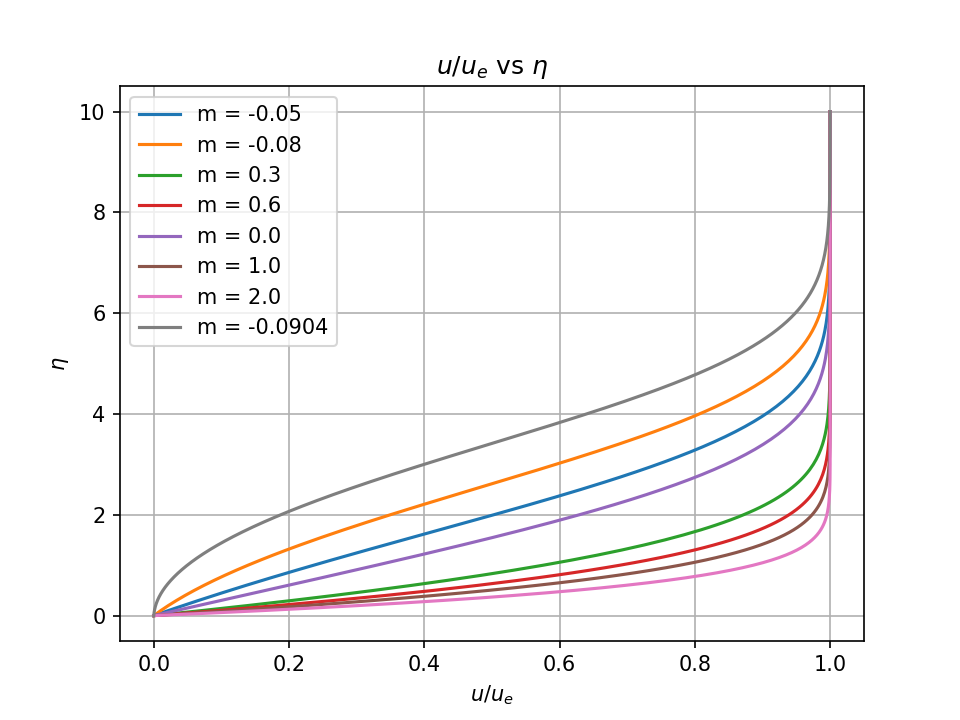
\includegraphics[scale=0.5]{supporting_documents/02_question_2_and_3_codeDevelopment/03_postProcessing/plot_1.png}
    \caption{streamwise velocity profiles plot for different m values}
    \label{plot_1}
\end{figure}

\par The streamwise velocity profile variations for different m values can
be found in \Cref{plot_1}. From the graph, it can be seen that as the
m value increases, the gradient of velocity is also increased. The velocity
profile for $m = -0.09043$ shows, the edge of separation.


\begin{figure}[!h]
   \centering
    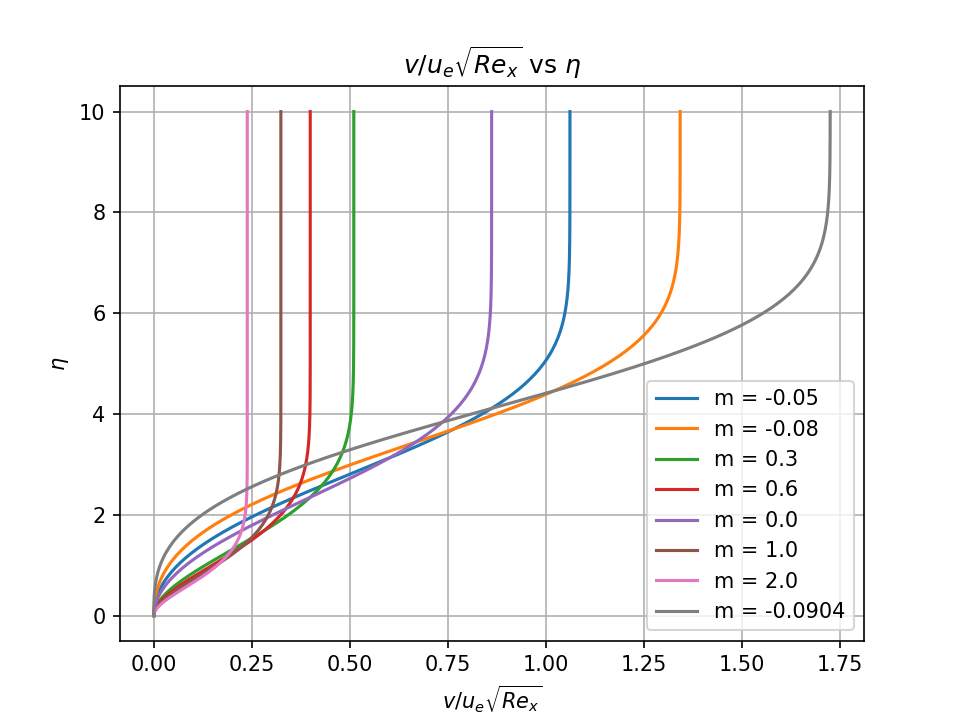
\includegraphics[scale=0.5]{supporting_documents/02_question_2_and_3_codeDevelopment/03_postProcessing/plot_2.png}
    \caption{normal velocity profiles plot for different m values}
    \label{plot_2}
\end{figure}

\par The normal velocity profiles given in \Cref{plot_2} for different m values
show that the normal velocity decreases with increase in m value, indicating
the change in wedge angle for the given flow.\\

\begin{figure}[!h]
   \centering
    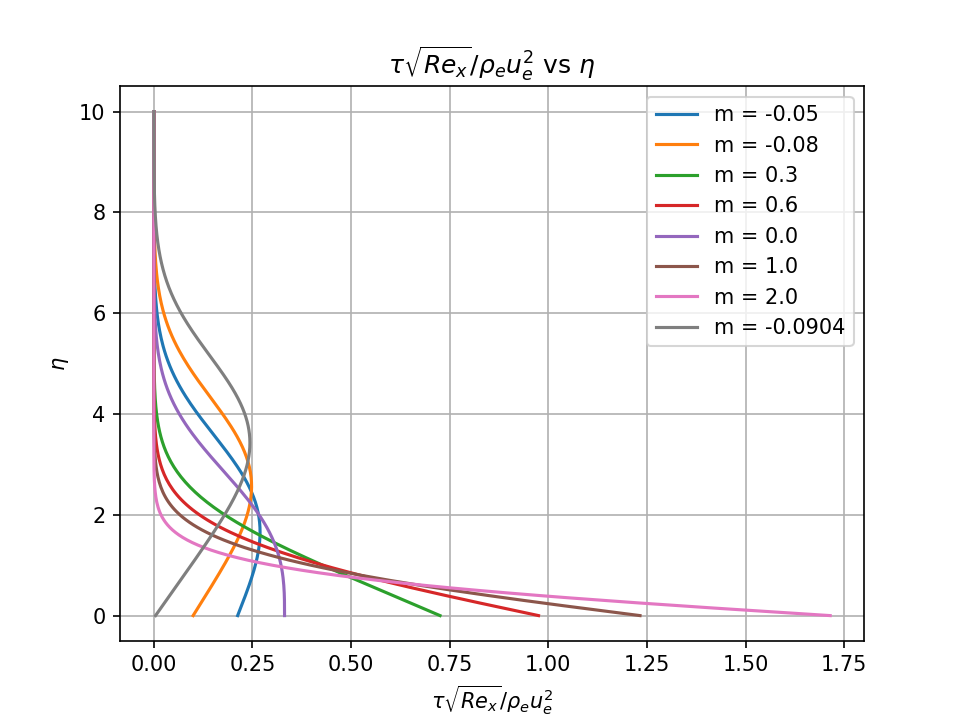
\includegraphics[scale=0.5]{supporting_documents/02_question_2_and_3_codeDevelopment/03_postProcessing/plot_3.png}
    \caption{shear stress profiles for different values of m}
    \label{plot_3}
\end{figure}

\par The shear stress profiles given in \Cref{plot_3} show the inflection of
profile for the m values less than 0, indicating a favourable shear stress
gradient for the flow, till the point of separation where the adverse pressure
gradient dominates the shear stress gradient.

\pagebreak

\subsection{Table of derived variables}

\par In this section, the computed variables i.e. $f$, $f^{\prime}$, $f^{\prime\prime}$, $f^{\prime\prime\prime}$
were used in obtaining values for derived variables given below.\\

\(\frac{\delta^*}{\delta_{FS}}\): \\
This parameter gives the nondimensional displacement thickness for the given
flow field. The value for this is obtained from solution variables as given
in \Cref{d_star_dFS}.
\begin{align}
    \delta^* &= \int{}{} \left(1 - \frac{u}{u_e}\right) dy \nonumber \\
    \frac{\delta^*}{\delta_{FS}} &= \int{}{}\left( 1 - f^{\prime}\right) d\eta \nonumber \\
    \frac{\delta^*}{\delta_{FS}} &= \left[\eta - f(\eta)\right]_0^{\eta_{max}} \label{d_star_dFS}
\end{align}

\par Similarly, the nondimensional momentum thickness is obtained by integration
and is given by \Cref{theta_dFS} and this has been solved by numerical integration.
\begin{align}
    \frac{\theta}{\delta_{FS}} &= \int{}{}\left(f^{\prime} - \left(f^\prime\right)^2\right)d\eta \label{theta_dFS}
\end{align}

\par And the nondimensional shearstress is obtained as \Cref{Rex_Cf}.
\begin{align}
    \tau &= \mu \frac{\partial u}{\partial y} \nonumber \\
    &= \mu u_e f^{\prime\prime}(\eta) \sqrt{\frac{u_e}{\nu x}} \nonumber \\
    \frac{\tau \sqrt{Re_x}}{\rho_e u_e^2} &= f^{\prime\prime}(\eta) \nonumber \\
    \frac{1}{2}C_f \sqrt{Re_x} &= f^{\prime\prime}(\eta)|_{@wall} \label{Rex_Cf}
\end{align}

\par The expressions for $\lambda$ and $\tau$ are given in \Cref{lambda,Tau}.
\begin{align}
    \lambda &= \frac{\theta^2}{\nu} \frac{d u_e}{dx} = m \left(\frac{\theta}{\delta_{FS}}\right)^2 \label{lambda} \\
    \tau &= Re_{\theta}\frac{C_f}{2} = \left(\frac{\theta}{\delta_{FS}}\right)^2 f^{\prime\prime} \label{Tau}
\end{align}

\par The values obtained for above variabeles for each m value are given in \Cref{table_f}. And
their comparison plots were given in \Cref{FS_numerical_plot}, the computed data
were compared against the book data given in \cite{ref_2} to show the
accuracy of computation.

\begin{table}
   \centering
    \caption{Falkner-Skan Equation's derived solution variables}
    \label{table_f}
    \begin{tabular}{|c|c|c|c|c|c|c|c|}
    \hline
        m & $\frac{\delta^*}{\delta_{FS}}$ & $\frac{\theta}{\delta_{FS}}$ & H & $\sqrt{Re_x}\frac{C_f}{2}$ & $\lambda$ & $\tau$ & $F_\theta$ \\ \hline
    -0.0904 & 3.45079 & 0.86796 & 3.97577 & 0.00433 & -0.0681 & 0.00376 & 0.82145 \\ \hline
    -0.08 & 2.68541 & 0.83128 & 3.23047 & 0.09964 & -0.05528 & 0.08283 & 0.74395 \\ \hline
    -0.05 & 2.12304 & 0.75256 & 2.82108 & 0.21247 & -0.02832 & 0.15989 & 0.59283 \\ \hline
    0.0 & 1.72351 & 0.66485 & 2.59233 & 0.33138 & 0.0 & 0.22032 & 0.44064 \\ \hline
    0.3 & 1.02025 & 0.44203 & 2.30809 & 0.72548 & 0.05862 & 0.32069 & 0.13631 \\ \hline
    0.6 & 0.79799 & 0.35472 & 2.24962 & 0.97514 & 0.0755 & 0.3459 & 0.05015 \\ \hline
    1.0 & 0.64822 & 0.29212 & 2.21902 & 1.23239 & 0.08533 & 0.36 & -4e-05 \\ \hline
    2.0 & 0.47682 & 0.21739 & 2.19343 & 1.71443 & 0.09451 & 0.37269 & -0.04728 \\ \hline
    \end{tabular}
\end{table}

\begin{figure}[!h]
    \begin{subfigure}{0.45\linewidth}
       \centering
        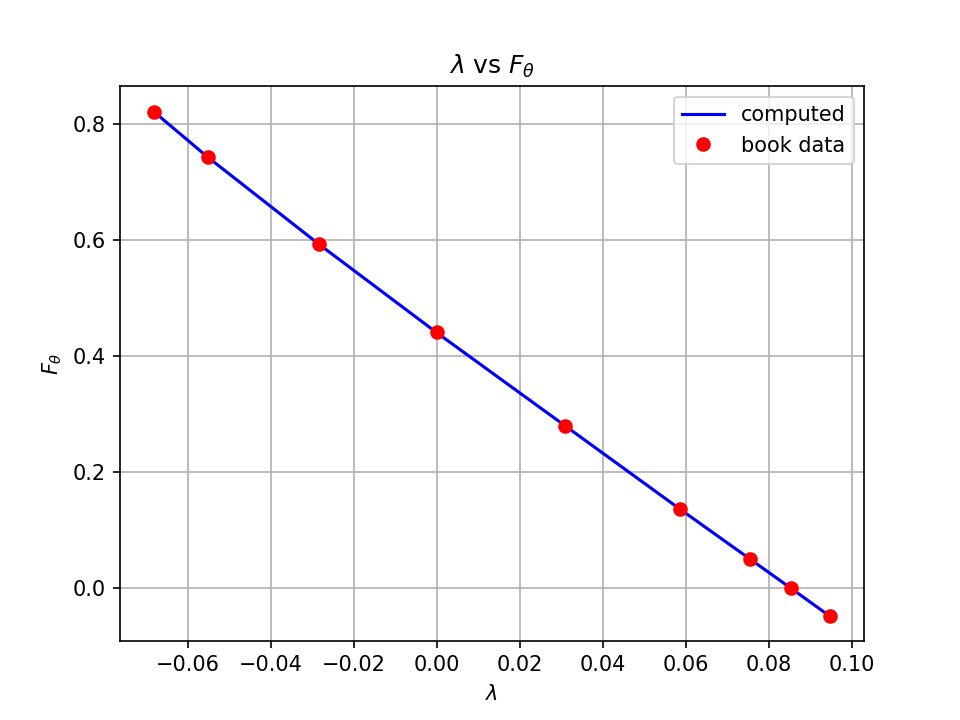
\includegraphics[scale=0.5]{supporting_documents/02_question_2_and_3_codeDevelopment/03_postProcessing/lambda_vs_F_theta.png}
        \caption{$\lambda$ vs $F_\theta$}
    \end{subfigure}
    \hfill
    \begin{subfigure}{0.45\linewidth}
       \centering
        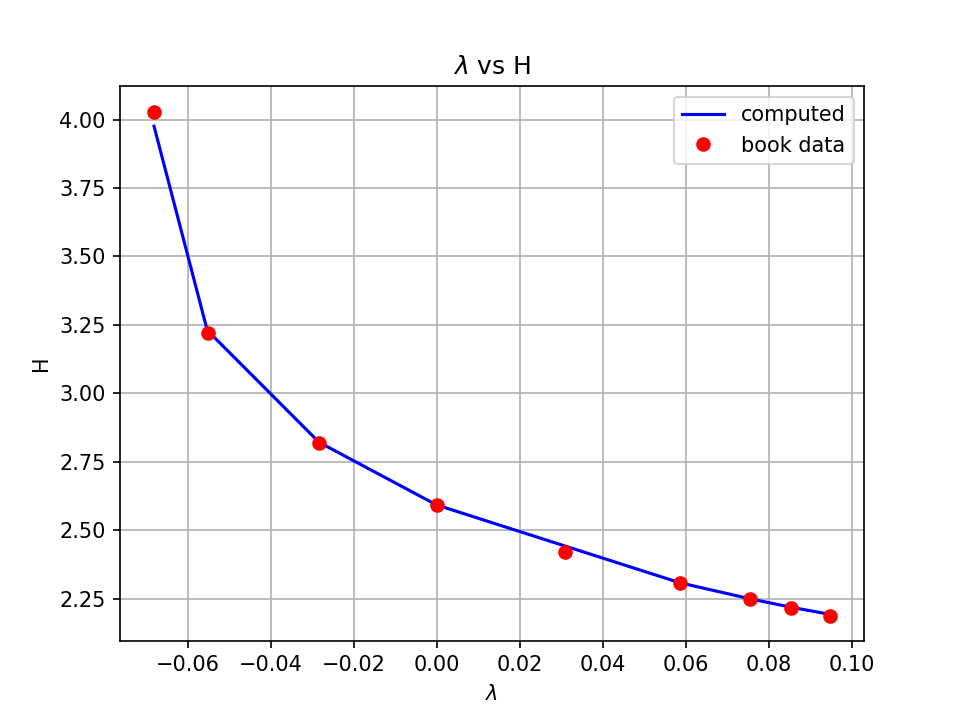
\includegraphics[scale=0.5]{supporting_documents/02_question_2_and_3_codeDevelopment/03_postProcessing/lambda_vs_H.png}
        \caption{$\lambda$ vs H}
    \end{subfigure}
    \hfill
    \begin{subfigure}{1.00\linewidth}
       \centering
        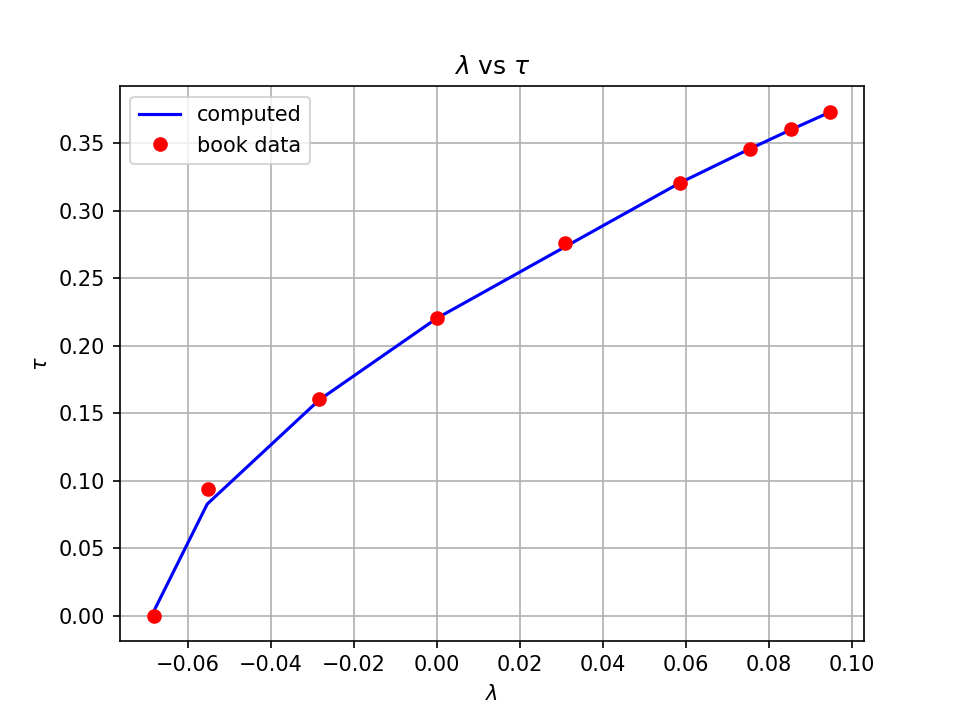
\includegraphics[scale=0.5]{supporting_documents/02_question_2_and_3_codeDevelopment/03_postProcessing/lambda_vs_Tau.png}
        \caption{$\lambda$ vs $\tau$}
    \end{subfigure}
    \caption{Variation of derived parameters vs $\lambda$}
    \label{FS_numerical_plot}
\end{figure}
